\documentclass[a4paper, 12pt,twoside]{book}

% set the paper size and the margins
\usepackage[top = 2cm, bottom = 2cm, left = 2cm, right = 4cm ]{geometry}
\usepackage[showboxes]{textpos}
\setlength{\TPHorizModule}{10mm}
\setlength{\TPVertModule}{\TPHorizModule}
\TPMargin{2mm}
% set the header and the footnote
\usepackage{fancyhdr}
% Supress the hyphenation
\hyphenation{thatshouldnot}
% for table and equations
\usepackage{tablefootnote}
\usepackage{amsmath,amsfonts,amsthm}
\usepackage{multirow}
\usepackage{hhline}
% make a wide hat for the least-squares regression line
 \usepackage{scalerel,stackengine}
\stackMath
\newcommand\reallywidehat[1]{%
\savestack{\tmpbox}{\stretchto{%
  \scaleto{%
    \scalerel*[\widthof{\ensuremath{#1}}]{\kern-.6pt\bigwedge\kern-.6pt}%
    {\rule[-\textheight/2]{1ex}{\textheight}}%WIDTH-LIMITED BIG WEDGE
  }{\textheight}% 
}{0.5ex}}%
\stackon[1pt]{#1}{\tmpbox}%
}
\usepackage[shortlabels]{enumitem}

% knitr packages
\usepackage[]{graphicx}
\usepackage[]{color}
%% maxwidth is the original width if it is less than linewidth
%% otherwise use linewidth (to make sure the graphics do not exceed the margin)
\makeatletter
\def\maxwidth{ %
  \ifdim\Gin@nat@width>\linewidth
    \linewidth
  \else
    \Gin@nat@width
  \fi
}
\makeatother

\definecolor{fgcolor}{rgb}{0.345, 0.345, 0.345}
\newcommand{\hlnum}[1]{\textcolor[rgb]{0.686,0.059,0.569}{#1}}%
\newcommand{\hlstr}[1]{\textcolor[rgb]{0.192,0.494,0.8}{#1}}%
\newcommand{\hlcom}[1]{\textcolor[rgb]{0.678,0.584,0.686}{\textit{#1}}}%
\newcommand{\hlopt}[1]{\textcolor[rgb]{0,0,0}{#1}}%
\newcommand{\hlstd}[1]{\textcolor[rgb]{0.345,0.345,0.345}{#1}}%
\newcommand{\hlkwa}[1]{\textcolor[rgb]{0.161,0.373,0.58}{\textbf{#1}}}%
\newcommand{\hlkwb}[1]{\textcolor[rgb]{0.69,0.353,0.396}{#1}}%
\newcommand{\hlkwc}[1]{\textcolor[rgb]{0.333,0.667,0.333}{#1}}%
\newcommand{\hlkwd}[1]{\textcolor[rgb]{0.737,0.353,0.396}{\textbf{#1}}}%
\let\hlipl\hlkwb
\usepackage{framed}
\makeatletter
\newenvironment{kframe}{%
 \def\at@end@of@kframe{}%
 \ifinner\ifhmode%
  \def\at@end@of@kframe{\end{minipage}}%
  \begin{minipage}{\columnwidth}%
 \fi\fi%
 \def\FrameCommand##1{\hskip\@totalleftmargin \hskip-\fboxsep
 \colorbox{shadecolor}{##1}\hskip-\fboxsep
     % There is no \\@totalrightmargin, so:
     \hskip-\linewidth \hskip-\@totalleftmargin \hskip\columnwidth}%
 \MakeFramed {\advance\hsize-\width
   \@totalleftmargin\z@ \linewidth\hsize
   \@setminipage}}%
 {\par\unskip\endMakeFramed%
 \at@end@of@kframe}
\makeatother


\definecolor{shadecolor}{rgb}{.97, .97, .97}
\definecolor{messagecolor}{rgb}{0, 0, 0}
\definecolor{warningcolor}{rgb}{1, 0, 1}
\definecolor{errorcolor}{rgb}{1, 0, 0}
\newenvironment{knitrout}{}{} % an empty environment to be redefined in TeX

\usepackage{alltt}


% packages will be used by the 'kable' package
\usepackage{booktabs}
\usepackage{longtable}
\usepackage{array}
\usepackage{multirow}
\usepackage[table]{xcolor}
\usepackage{wrapfig}
\usepackage{float}
\usepackage{colortbl} 
\usepackage{pdflscape}
\usepackage{tabu}
\usepackage{threeparttable}
\usepackage{threeparttablex}
\usepackage[normalem]{ulem}
\usepackage{makecell}
\usepackage{xcolor}
\IfFileExists{upquote.sty}{\usepackage{upquote}}{}

% define a color for highlight
\definecolor{asparagus}{rgb}{0.53, 0.66, 0.42}
\definecolor{babypink}{rgb}{0.96, 0.76, 0.76}
\definecolor{champagne}{rgb}{0.97, 0.91, 0.81}
\definecolor{forestgreen}{rgb}{0.13, 0.55, 0.13}
\definecolor{dollarbill}{rgb}{0.52, 0.73, 0.4}

\usepackage{tcolorbox}

\tcbset{width=0.9\textwidth,boxrule=0pt,colback=champagne,arc=0pt,
auto outer arc,left=0pt,right=0p}

\usepackage{hhline}

\begin{document}

%Deal with the headers of each chapter
\pagestyle{fancy}
\fancyhf{}
\renewcommand{\chaptermark}[1]{ \markboth{#1}{} }
\fancyhead[CE,CO]{\leftmark}
\fancyfoot[LE,RO]{\thepage}

\chapter{Designing studies}

In this chapter we will learn two ways to acquire data: sampling and experiments. Both of them should be designed carefully to make sure the conclusions derived from them are persuasive.
\newpage

\section{Sampling}
 
\textbf{\large{Basic concepts and ideas}}
\vspace{0.3cm}

Sampling is a kind of observational study. It doesn't interfere the subjects to be studied. For example, you want to know the average household income in China, you can sample 10,000 out of all the households and make a record of their yearly income. During this process, you just "record" without influencing their income. 
\vspace{0.3cm}

All the households in China is called the \textbf{population}, and the 10,000 household sampled out is called a \textbf{sample}. If you recorded the data of all the households in China, then this process is called \textbf{census}.
\vspace{0.3cm}

The reason of sampling is to draw conclusions about the population, thus the sample should be representative. The first step in planning a \textbf{sampling survey} is to say exactly \textit{ what population} we want to describe. The second step is to say exactly \textit{what we want to measure}, that is, to point out the variable we want to measure.
\vspace{0.6cm}\\
\textbf{\large{Bias and sources of bias}}
\vspace{0.3cm}

For a bad sample, it consistently overestimates or underestimates the value, and this phenomenon is called \textbf{bias}.
\vspace{0.3cm}

Good samples sometimes overestimate and sometimes underestimate the value of the variable to be estimated, and this variability is called \textbf{sampling errors}. But they never "consistently" overestimate or underestimate.
\vspace{0.3cm}

There are many sources of bias. Although each of the following sources of bias are defined separately, there is overlap, and many if not most examples of bias involve more than one of the following.

    \begin{enumerate}
       \item   \textbf{Convenience sample} is a sample generated by choosing easy-to-reach individuals from a population. For example, to estimate the percentage of high school students who have graphing calculators, you draw a sample from our statistics class for convenience. Obviously, this sample is biased and it tends to overestimate the percentage of students with calculators.
       
       \item \textbf{Voluntary response bias} is generated by letting the individuals participate the survey voluntarily. Often those with strong opinions are more likely to participate, leading to an over emphasis of those individuals. For example, a radio call-in program about whether should each one get a house for free.
       
       \item \textbf{Undercoverage bias} happens when some individuals do not have equal chance to be selected. Telephone survey will ignore those who do not have telephones.
       
       \item \textbf{Nonresponse bias} happens when some of the chosen individuals refuse to respond. Those unresponsive individuals may hold some particular opinions and they are ignored.
       
       \item \textbf{Response bias} happens when participants give unfaithful answers. For example, no participants will say they are a criminal in a survey to estimate the percentage of criminals in the population.
       
       \item \textbf{Wording bias} is caused by poorly worded question. Here is an interesting example.
       \begin{center}
       \begin{minipage}{0.8\textwidth}
       It is estimated that disposable diapers account for less than 2\% of the trash in today’s landfills. In contrast, beverage containers, third-class mail, and yard wastes are estimated to account for about 21\% of the trash in landfills. Given this, in your opinion, would it be fair to ban disposable diapers?
       \end{minipage}
       \end{center}
     Do you think it has a wording bias?
    \end{enumerate}

\colorbox{babypink}{\parbox{\textwidth}{
In AP exam, if asked to describe how the design of a study leads to bias, you should \textbf{(1) identify the bias and (2) explain how the design leads to underestimation or overestimation}. For a design as "Draw a sample from your AP statistics class to estimate the percentage of students with calculators", you may say "It is an convenience sample and it tend to overestimate the percentage, because all the students in the AP statistics class are required to have a graphing calculator."
}}
\vspace{0.3cm}

\textbf{\large{Good samples}}
\vspace{0.3cm}

\begin{enumerate}

\item \textbf{Simple Random Sample(SRS)} of size $n$ is chosen in such a way that every group of $n$ individuals in the population has an equal chance to be selected as the sample.

\textbf{Steps:}
   \begin{enumerate}[(1)]
       \item \textbf{Label.} Give each individual in the population a distinct number.
       \item \textbf{Randomize.} Use random number number generator or \textit{table of random digits} to generate $n$ distinct numbers
       \item \textbf{Choose.} Put the individuals corresponding to the selected  number in the previous in the sample
   \end{enumerate}
   \vspace{0.3cm}
   
\item \textbf{Systematic sample.} For example, you want sample 10 individuals out of a population of 100 systematically. The procedures will be:
    \begin{enumerate}[(1)]
        \item Label the individuals in the population from 1 to 100.
        \item Randomly choose a number from 1 to 10, let's say it is 6.
        \item Pick every tenth number following 6. They are 16, 26, ... , 96
        \item Select the individuals corresponding to the above numbers as a systematic sample.
    \end{enumerate}
    \vspace{0.3cm}
    
\item \textbf{Stratified Random Sample} is generated first by dividing the population into \textit{homogeneous} groups called \textit{strata}, selecting SRS from each stratum, then combining all those SRS together. 
\vspace{0.3cm}

For example, you want investigate the hair length of all the students in a high school, you can divide the students into two strata by gender, since gender strongly influence the hair length, and the hair length in each group can be considered \textit{homogeneous}. Then draw SRS from each group, and combine those two SRS together to form a stratified random sample.
\vspace{0.3cm}

\begin{textblock}{3}(15.5, -4)
\textblockcolor{dollarbill}
\noindent
Is \textit{stratified random sample} simple random sample?\\
\end{textblock}

\item \textbf{Cluster sample} is generated by dividing the population into \textit{heterogeneous} groups called \textit{clusters}, then randomly select clusters from among all clusters. 
\vspace{0.3cm}

In previous example, instead of dividing the students by gender, we divide the students into classes. The hair length in each class is \textit{heterogeneous} and can be considered as a miniature of the population. Each class is called a cluster. We randomly choose classes from among all the classes and combine the chosen classes to form a cluster sample.
\end{enumerate}
\vspace{0.3cm}

\begin{textblock}{3}(-3, -4)
\textblockcolor{dollarbill}
\noindent
Is \textit{cluster sample} simple random sample?\\
\end{textblock}


\colorbox{champagne}{\parbox{0.95\textwidth}{

    \textbf{Exercise}
    
    A British farmer grows sunflowers for making sunflower oil. Her field is  arranged in a grid pattern, with 10 rows and 10 columns as shown in the  figure on the next page. Irrigation ditches run along the top and bottom of the field. The farmer would like to estimate the number of healthy plants in the field so she can project how much money she’ll make from selling them. It would take too much time to count the plants in all 100 squares, so she’ll accept an estimate based on a sample of 10 squares.
    
    \begin{figure}[H]
        \centering
        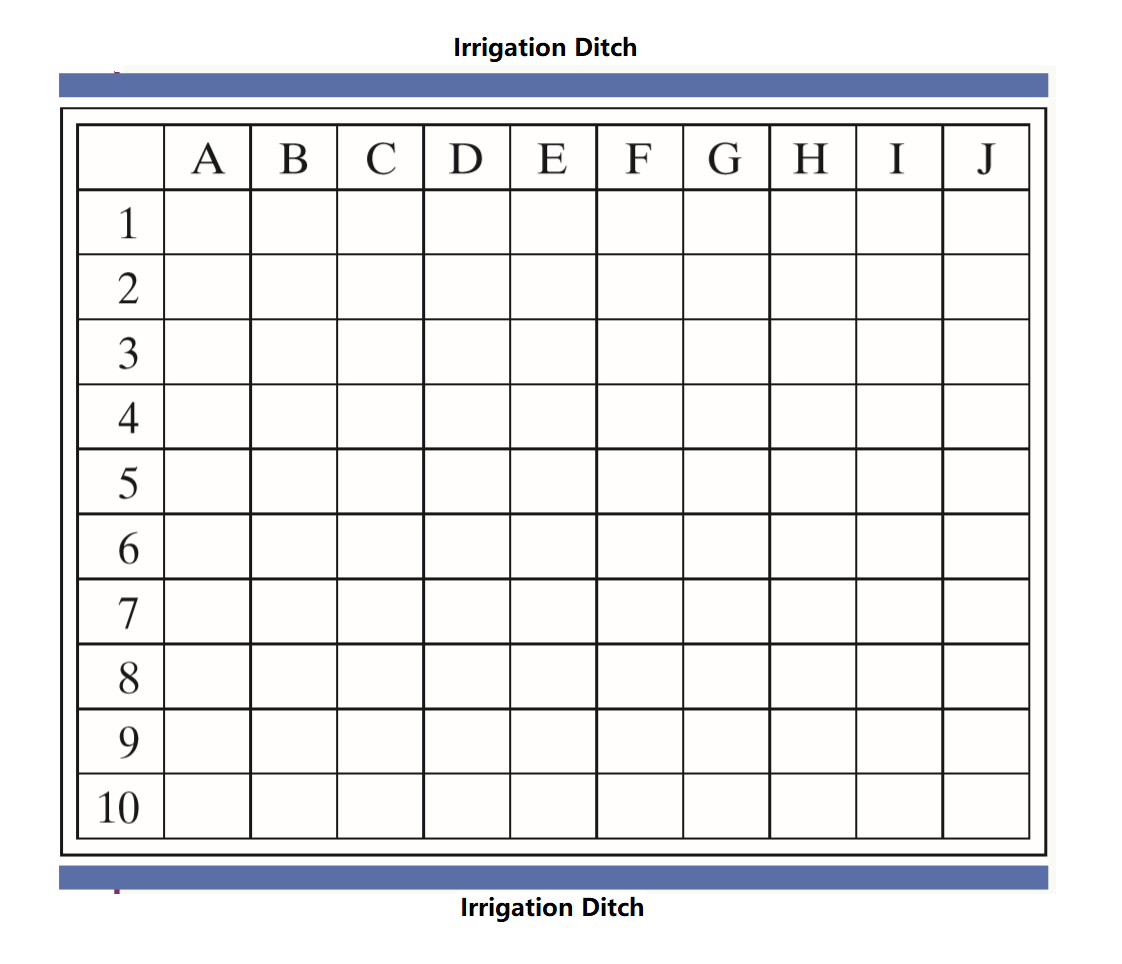
\includegraphics[scale=0.3]{Sunflower}
    \end{figure}

Give the sampling method for
   \begin{enumerate}[(a)]
       \item simple random sample(SRS)
       \item systematic sample
       \item cluster sample 
       \item stratified random sample
       \item In (c) why do you cluster the population that way?
       \item In (d) why do you stratify the population that way?
   \end{enumerate}
}}
\newpage

\textbf{\large{The advantages of stratified random sample}}
\vspace{0.3cm}

Let's use the previous exercise as an example. If we draw SRS many times, some of the samples may fall in the middle of the field(circle \textbf{L}), which is far away from the irrigation  ditches, and consequently gives lower estimations of the production of sunflower seeds. Some samples may fall near the irrigation ditch(\textbf{circle \textbf{H}}) and give higher estimations of the production of sunflower seeds. Figure \ref{CompareSRSandStratifiedRS} gives the distribution of 100 samples of SRS and stratified random samples. Each dot represents a sample.

    \begin{figure}[H]
        \centering
        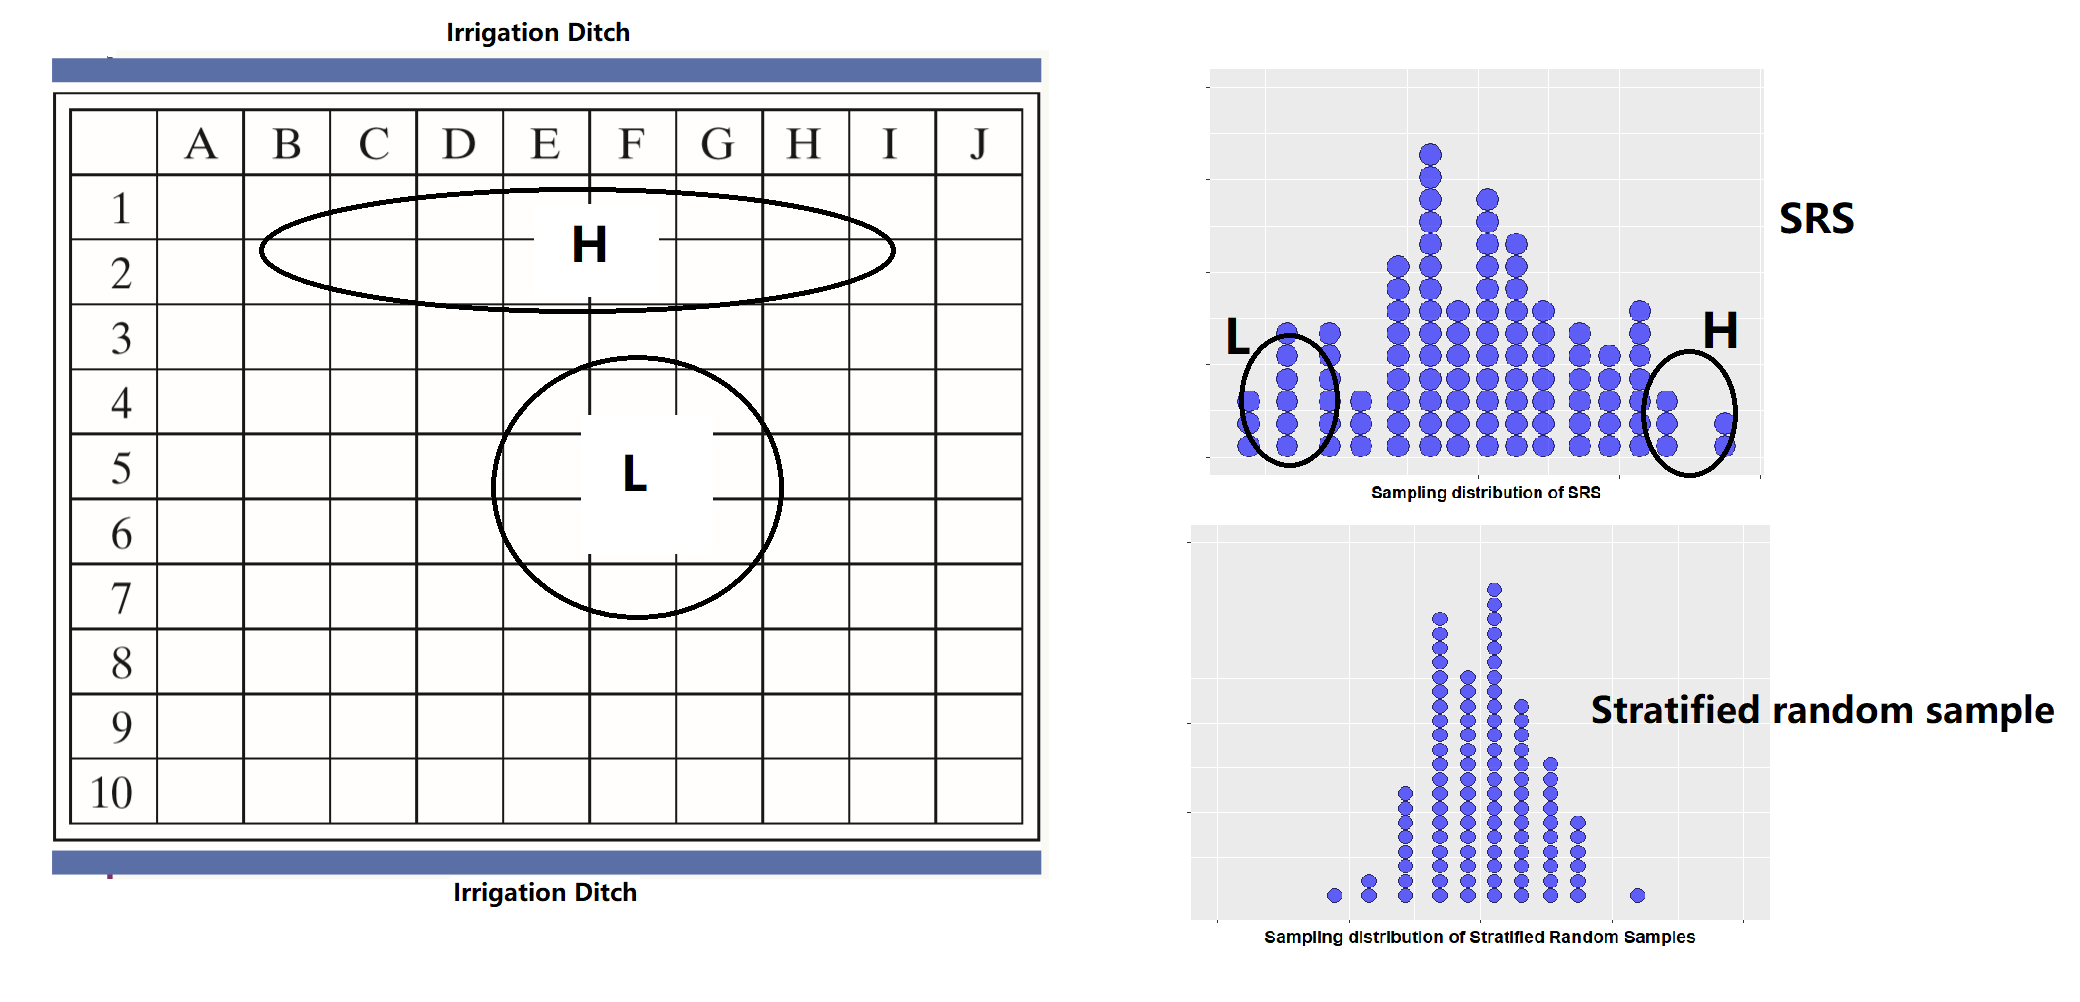
\includegraphics[scale=0.4]{CompareSRSandStratifiedRS}
        \caption{Compare SRS and stratified random sample
                \label{CompareSRSandStratifiedRS}}
    \end{figure}
    
    However, the extreme cases as circle \textbf{L} and circle \textbf{H} never happen for stratified random samples. The estimations based on stratified random samples have less variation than estimations based on simple random samples. 
    \vspace{0.3cm}
    
    \colorbox{babypink}{\parbox{\textwidth}{    
        Stratified random sample can reduce the variation of the estimations than SRS.
    }}
    \newpage
    
\section{Experiments}


In an \textbf{observational study}, we can only come to the conclusion about \textit{association}, not \textit{cause and effect} or \textit{causation} relation. For example, every day you get up, you see the rises. There is an \textit{association} between "you get up" and the "sun rises", but you can not say the "sun rises" because "you get up".
\vspace{0.3cm}

The reason why we can not come to the conclusion of \textit{cause and effect} is because we can not rule out the influence of other factors, such as the rotation of the earth. If you make another observational study, you may find the "rotation of the earth" and the "sun rises" are closely associated as well. When we can not distinguish the effect of more than one variable on a response variable, we say there is a \textbf{confounding}.
\vspace{0.3cm}\\

\noindent
\colorbox{babypink}{\parbox{\textwidth}{
   The observational studies can not come to conclusions about causations because of confounding. 
   \textbf{Experiments can exclude confounding effect and give conclusions about cause and effect.}
}}
\vspace{0.3cm}

\vspace{0.6cm}

\textbf{\large{Principles of Experimental design}}
\vspace{0.3cm}

Now, we developed a new painkiller. We want to do some experiments to test whether it is more effective than the existing one. 
\vspace{0.3cm}

    \begin{enumerate}[(1)]
        \item \textbf{Comparison.} We have to compare the effectiveness of the new painkiller with with the existing one.
        \item \textbf{Random assignment.} We have to randomly assign the \textbf{subjects} into different \textbf{treatments:} one treatment is to take the new painkiller, the other treatment is to take the existing painkiller. 
        \vspace{0.3cm}
        
        \colorbox{babypink}{\parbox{0.9\textwidth}{
The purpose of \textit{random assignment} is to make the subjects allocated to different treatments are roughly the same, and thus rule out \textit{confounding}.
}}
\vspace{0.3cm}
        
 For example, if we allocate those with heavy body weight to the treatment of taking new painkiller, and the others to take the existing painkiller, we don't know whether the relief of pain is caused by body weight or the effectiveness of the new drug, and lead to \textit{confounding}. Beside the observable factors, such as body weight, there are unobservable factors that may influence the outcome as well. Random assignment can also even out those unobservable factors.
        \item \textbf{Control} is to keep other variables that might affect the response the same. \textit{Random assignment} is a way to control.  Another way to control is  \textbf{blocking}. A \textbf{control} group receives no treatments while all other variables are the same as the groups that receive treatments
        \item \textbf{Blocking} is to divide the subjects into different groups by the factors that may strongly influence the outcome, and design experiments within each group. Those different groups are called \textbf{blocks}.
        \item \textbf{Replication} is to use enough \textbf{experimental units} in each group so that any difference in the effects of the treatments can be distinguished from chance variance between groups.
        \vspace{0.3cm}
        
    For example, we only have two subjects, and each one is randomly assigned to take either the new or existing painkiller, and it happens that the new painkiller is more effective. People may argue that the one assigned to take the new painkiller happens to be more resistant to pains and the effectiveness if not caused by the new drug. In this case, we can not rule out the influence of chance variance.  
    \end{enumerate}
    \vspace{0.3cm}
    
   \textbf{\large{Design experiments}}
   \vspace{0.3cm}
   
   \begin{enumerate}[(1)]
       \item \textbf{Completely randomized design}
       
   For example we have 80 subjects to test the effectiveness of the new painkiller. We can design the experiments in the following way.
   
       \begin{figure}[H]
           \centering
           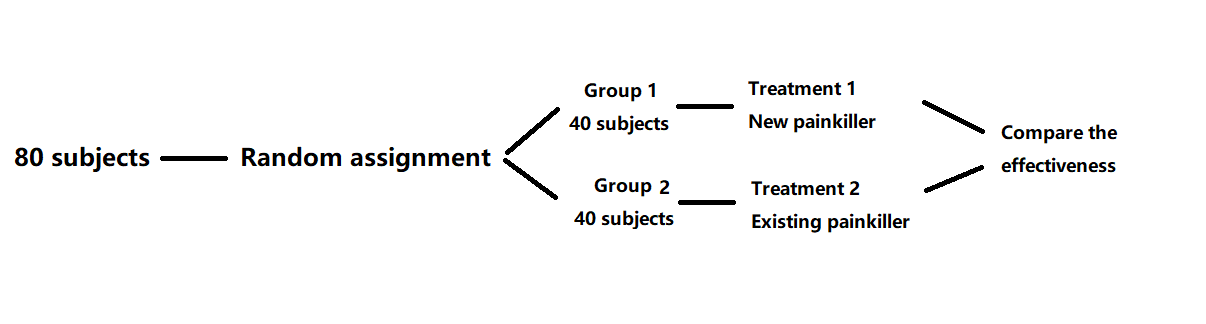
\includegraphics[scale=0.6]{CompletelyRandomizedDesign}
           \caption{Completely randomized design 
            \label{CompletelyRandomizedDesign}}
       \end{figure}
       The procedures are given as follows:
          \begin{enumerate}
              \item Assign numbers from 1 to 80 to those 80 subjects.
              \item Use random number generator to generate 40 distinct random numbers within 1 and 80
              \item The subjects corresponding to the 40 numbers in the above step go to group 1 and will take new painkillers. The other 40 subjects go to group 2 and will take existing painkiller.
              \item Compare the effectiveness between the two groups.
          \end{enumerate}
          \vspace{0.3cm}
     
     \colorbox{babypink}{\parbox{\textwidth}{
     \begin{enumerate}[\Roman*.]
         \item In AP exam, when you are asked to design an experiment, drawing the graph is not enough, you have to describe in detail how to carry out those procedures. Make sure people can carry out the experiment by following your design. You can not just say "random assignment", you have to describe how to do this "random assignment"
         
         \item Here I say compare the effectiveness. It is not good. In AP example you have to describe exactly what variable to be measured. In this example, it could be like "After they take the painkillers, punch them with equal strength, and measure the loudness of their cry and lower loudness means the medicine is more effective.        
     \end{enumerate}
     }} 
     \vspace{0.3cm}   
     
  \item \textbf{Randomized block design} 
  
  Now we have 80 subjects, 40 of the are male and 40 of them are female. And we know gender can strongly influence the effectiveness of the medicine. We can do a \textit{randomized block design} to rule out the confounding of gender in the following way.
  \begin{figure}[H]
      \centering
      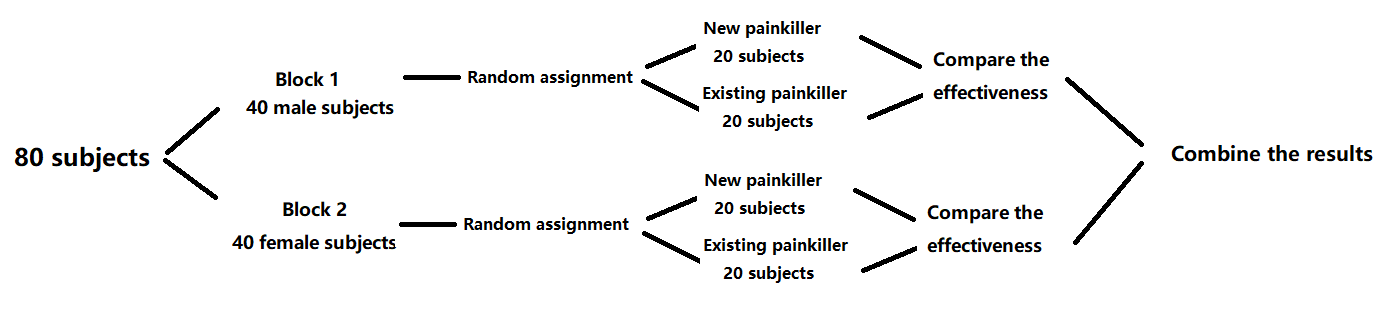
\includegraphics[scale=0.6]{RandomizedBlockDesign}
      \caption{Randomized block design 
      \label{RandomizedBlockDesign}}
  \end{figure}
  
\colorbox{champagne}{\parbox{0.9\textwidth}{
\textbf{Exercise}

 Describe in detail of the above \textit{randomized block design}.
 }}
 \newpage
 \item \textbf{Matched pairs design}
  \vspace{0.3cm}
  
  \textit{Matched pairs design} is a special type of randomized block design. In each block there are either two \textit{very similar} individuals or one individual with two measurements. 
  \vspace{0.3cm}
  
  \textbf{One individual with two measurements}
  \vspace{0.3cm}
  
  Now let's do a \textit{matched pairs design} to study whether the standing pulse rates generally higher than sitting pulse rates? Let's say the number of subjects is $n$.
  \vspace{0.3cm}
  
    \begin{enumerate}[(a)]
        \item \textbf{Let each subject randomly decide which treatment comes first and apply the treatment}. 
        
        For example, by throwing a coin, if it is a head, then measure the standing heart rates first, otherwise measure the sitting heart rates first.
        \item \textbf{Apply the other treatment that is not applied on each subject.} 
        
        In this example, for those who measured standing heart rates first, measure sitting heart rates this time. And for those who measured sitting heart rates first, measure the standing heart rate this time.
        \item \textbf{Compare each pair of the data acquired in previous steps(\textit{compare within block)}.} 
        
        Let $\{x_1, x_2, ..., x_n\}$ be the standing heart rates of the n subjects, and $\{y_1, y_2, ..., y_n\}$ be the corresponding sitting heart rates. We compare each pair of data by subtract $y_i$ from $x_i$, then we get a new set of data $\{x_1-y_1, x_2-y_2, ..., x_n-y_n\}$.
        \item\textbf{ Analyze the data generated from the previous step(\textit{combine the results from each block}). }
        
        We analyze data set $\{x_1-y_1, x_2-y_2, ..., x_n-y_n\}$ to see whether the standing heart rates is higher than the sitting heart rate(\textit{We will learn how to analyze those data in chapter about statistical inferences}).
    \end{enumerate}
    \vspace{0.3cm}
    
    \colorbox{babypink}{\parbox{0.95\textwidth}{
    \textbf{Remark:}
    
        \begin{enumerate}[\Roman*.]
            \item Randomizing the order of the treatments is to eliminate the confounding that the order of the treatment may influence the response variable.
            \item When you are asked to describe a matched pairs design, you are supposed to give details. The procedures given above are too general.
        \end{enumerate}
    }}
  \vspace{0.6cm}
    \newpage
    
    
  \textbf{Two individuals in each block}
  \vspace{0.3cm}
  
    \begin{minipage}{\textwidth}
    \hspace{-1cm}
  \colorbox{champagne}{\parbox{\textwidth}{
  
        \textbf{Exercise}
      \vspace{0.3cm}
      
      \textbf{Nitrogen in tires\textemdash a lot of hot air?}
 
   Most automobile tires are inflated with compressed air, which consists of about 78\% nitrogen. Aircraft tires are filled with pure nitrogen, which is safer than air in case of fire. Could filling automobile tires with nitrogen improve safety, performance, or both?     
   
   Consumers Union designed a study to test whether nitrogen-filled tires would maintain pressure better than air-filled tires. They obtained two tires from each of several brands and then filled one tire in each pair with air and one with nitrogen. All tires were inflated to a pressure of 30 pounds per square inch and then placed outside for a year. At the end of the year, Consumers Union measured the pressure in each tire. The amount of pressure lost (in pounds per square inch) during the year for the air-filled and nitrogen-filled tires of each brand is shown in the table below.
   \begin{figure}[H]
       \centering
       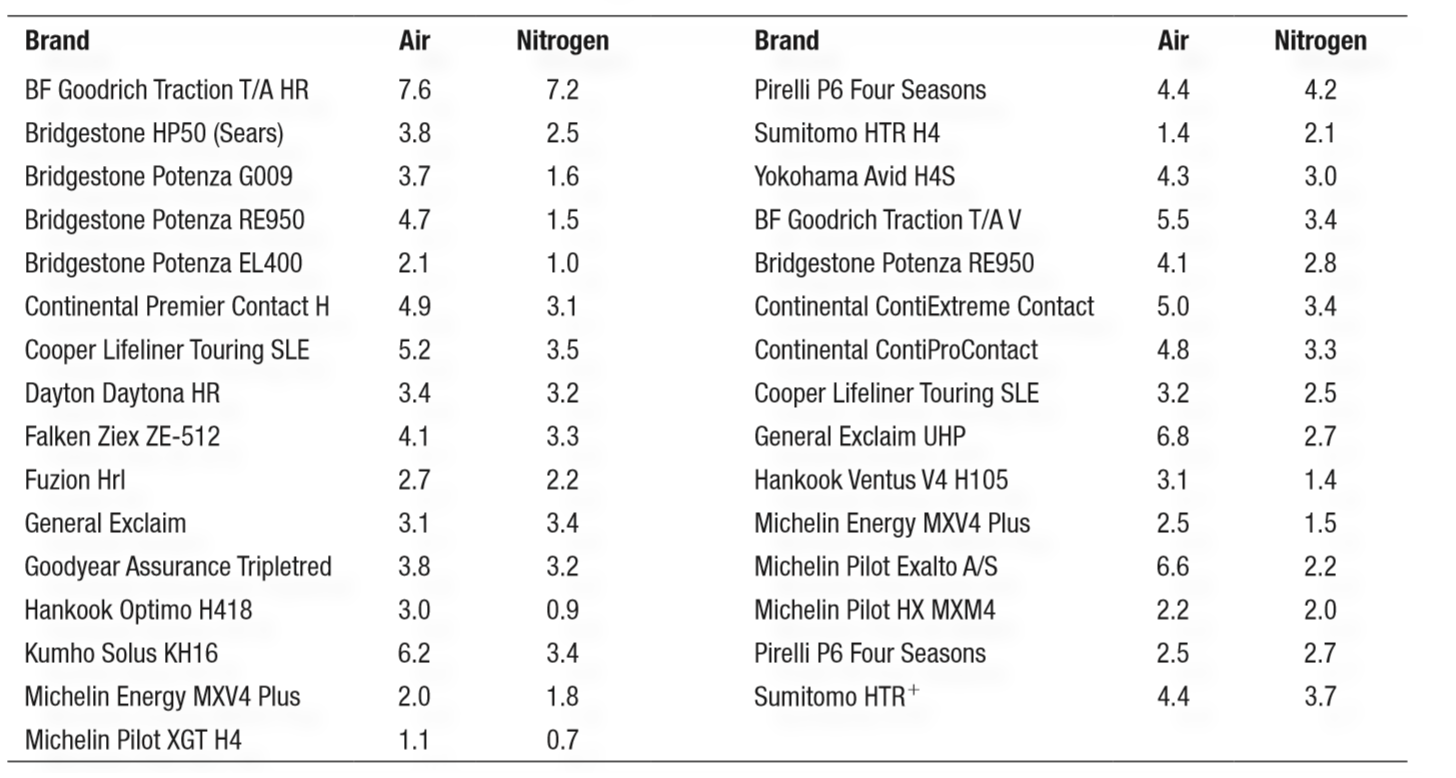
\includegraphics[scale=0.6]{MatchedPairsDesign}
       \caption{Matched pairs design}
       \label{MatchedPairsDesign}
   \end{figure}

  Does filling tires with nitrogen instead of compressed air reduce pressure loss? Give appropriate graphical and numerical evidence to support your answer.    
  }}
   \end{minipage}
   \newpage
   
   \item \textbf{Double blind}
   \vspace{0.3cm}
  
  The \textbf{Rosenthal effect} and \textbf{Self-fulfilling prophecy} tell us that what you think may influence the outcome. This phenomenon happens in experiments when the subjects are people. 
  
  Give a patient a sugar and tell him this is a painkiller, he may really feel that his pain is relieved after taking it. This is called \textbf{placebo effect}, and the sugar is a \textbf{placebo}.
  
  \textbf{Double-blind experiment} can exclude \textit{placebo effect}. In a \textit{double-blind experiment} neither the subjects nor those who interact with them and measure the response variable know which treatment a subject received.
  \vspace{0.3cm}
  
  \colorbox{babypink}{\parbox{0.92\textwidth}{
  \textit{Who knows which treatment a subject received?} People who design the experiment knows! Once a person knows which treatment a subject received, he should not participate in the procedure of measuring the response variable.
  }}
  \vspace{0.3cm}
  
 For example, there is a new drug to decrease blood pressure. To test whether it works or not we can do a \textit{double-blind experiment}. Randomly divide the subjects into two groups, one group is treated with real drug, the other is treated with placebo.  But all are told they are treated with drug. After they have taken the drug or placebo for a period of time, the blood pressure is measured by those who don't know whether the subject was fed with drug or placebos. 
 \vspace{0.3cm}
 
   \colorbox{babypink}{\parbox{0.92\textwidth}{
Sometimes double-blind experiment is impossible, we have to do single blind experiment.
  }}
  \vspace{0.3cm}
  
  For example we want to know whether diet or exercise is more effective in losing weight. No matter how the experiment is designed, the subjects will know what type of treatments they receive. But the people who measure the subjects' weight can be blind about the treatment each subject received. This type of experiment is called \textbf{single-blind experiment}.
  \vspace{0.3cm}
  \newpage
 
 \item \textbf{Conclusions and their generalization}
 \vspace{0.3cm}
 
 In order to draw conclusions, an observed effect need to be \textbf{statistically significant}, which means that the effect can rarely be explained by chance effect. 
 \vspace{0.3cm}
 
 Once the effect is statistically significant, what how far can we go about the inferences of the populations? What type of inference can we make?
 \vspace{0.3cm}
 
 Previously, we mentioned that observational study can not come to conclusions about \textit{cause and effect} relation because of confounding. When the experiment is designed without \textit{random assignment}, confounding can not be ruled out either, and \textit{cause and effect} relation can not be reached.
 \vspace{0.3cm}
 
 When subjects are not \textit{randomly selected}, they are not representative of the population, the conclusion drawn from those subjects can not be generalized to the population. 
 \vspace{0.3cm}
 
 The following table gives the scopes of inference on different occasions.
    
%     \begin{table}[H]
%     \hspace{-3cm}
%     \begin{tabular}{cccc}
%     \hline
%     &&\multicolumn{2}{c}{\textbf{Were individuals randomly assigned to groups?}}\\
%     \hhline{~~--}
%     &&\textbf{Yes}&\textbf{No}\\
%     \multirow{4}{*}{
%     \begin{minipage}{4cm}
%     \textbf{Were individuals  randomly selected?}
%     \end{minipage}
%     }
%     &\multirow{2}{*}{\textbf{Yes}}&Inference about the population :YES&Inference about the population:YES\\
%     &&Inference about cause and effect:YES&Inference about cause and effect:NO\\
%     \hhline{~---}
%     &\multirow{2}{*}{\textbf{No}}&Inference about the population: NO&Inference about the population: NO\\
%     &&Inference about cause and effect:YES&Inference about cause and effect:NO\\
%     \hline     
%     \end{tabular}
%     \end{table}
 
 \begin{figure}[H]
   \hspace{-2.5cm}
   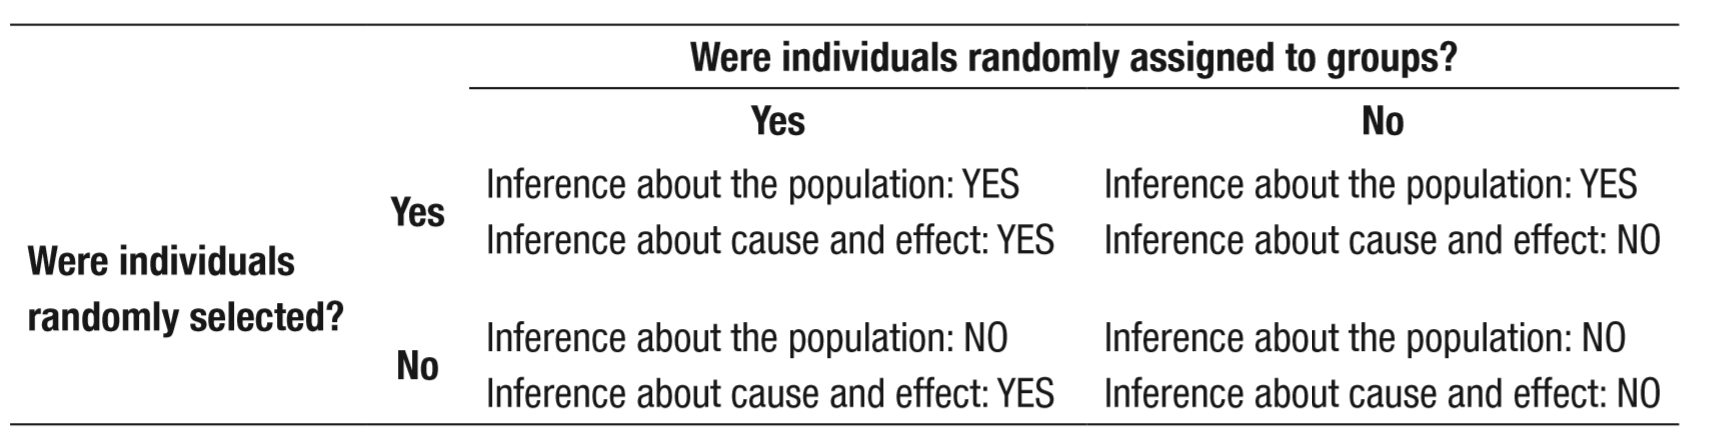
\includegraphics[scale=0.6]{ScopeOfInference}
   \label{ScopeOfInference}
 \end{figure}
 
 \end{enumerate}
 \newpage
 
 

   \colorbox{champagne}{\parbox{\textwidth}{
   \textbf{Vitamin C and Canker Sores}
   \vspace{3pt}
   
   A small-town dentist wants to know if a daily dose of 500 milligrams (mg) of vitamin C will result in fewer canker sores in the mouth than taking no vitamin C.
   \vspace{0.3cm}
   
   The dentist is considering the following four study designs:
   \vspace{0.3cm}
   
   \textit{Design 1}: Get all dental patients in town with appointments in the next two weeks to take part in a study. Give each patient a survey with two questions: (1) Do you take at least 500 mg of vitamin C each day? (2) Do you frequently have canker sores? Based on patients’ answers to Question 1, divide them into two groups: those who take at least 500 mg of vitamin C daily and those who don’t.
   \vspace{0.3cm}
   
   \textit{Design 2}: Get all dental patients in town with appointments in the next two weeks to take part in a study. Randomly assign half of them to take 500 mg of vitamin C each day and the other half to abstain from taking vitamin C for three months.
   \vspace{0.3cm}
   
   \textit{Design 3}: Select a random sample of dental patients in town and get them to take part in a study. Divide the patients into two groups as in Design 1.
   \vspace{0.3cm}
   
   \textit{Design 4}: Select a random sample of dental patients in town and get them to take part in a study. Randomly assign half of them to take 500 mg of vitamin C each day and the other half to abstain from taking vitamin C for three months.
   \vspace{0.3cm}
   
   For whichever design the dentist chooses, suppose she compares the proportion of patients in each group who complain of canker sores. Also suppose that she finds a statistically significant difference, with a smaller proportion of those taking vitamin C having canker sores.
   \vspace{0.3cm}
   
   \textbf{\textit{What can the dentist conclude for each design?}}
   
   
   
   }}
 


\end{document}